

\begin{comment}
 In the second test, we prove the functionality of the algorithm in three dimensions. 

The algorithm compares the images and calculates the departure factor 
based on area of ROI. Fig. \ref{fig:target} demonstrates the 
tracking of $40$ images from initial position to the final position of the target, 
highlighted with red boxes;
the vector in blue describes the movement of the target. 

\begin{figure}[H]
\centering
  \subfloat[]{\label{fig:targeinit} 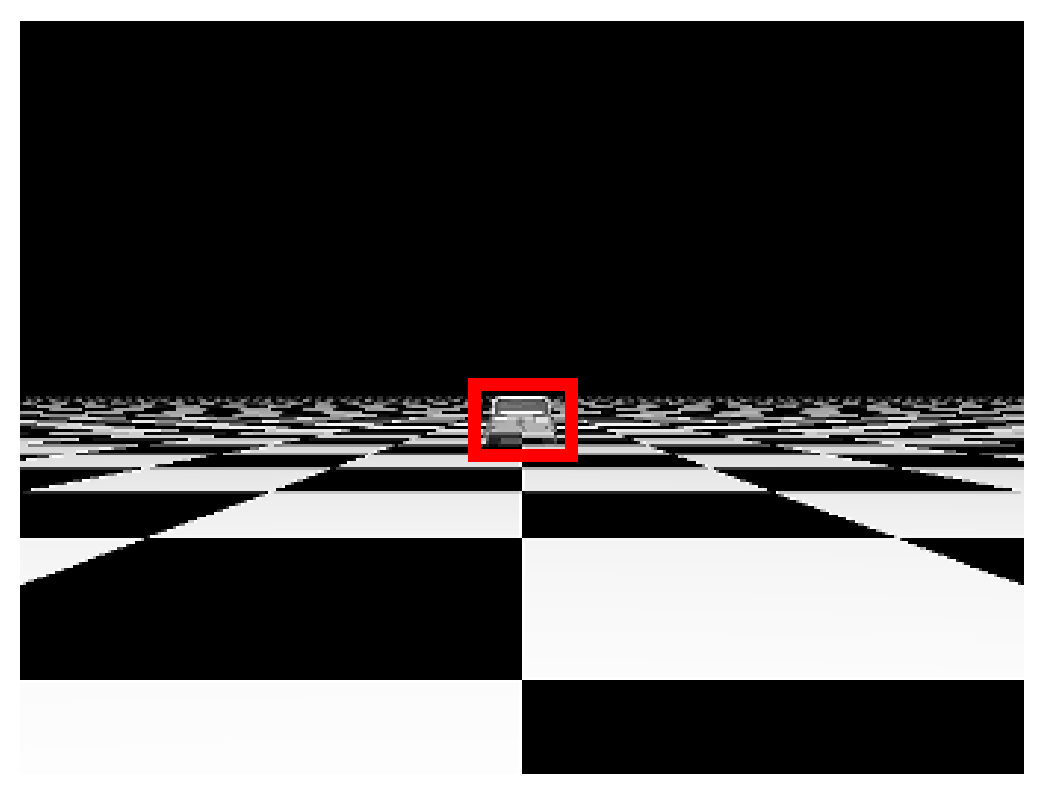
\includegraphics[width=.48\columnwidth]{images/figurea.eps}}
  \subfloat[]{\label{fig:targeend} 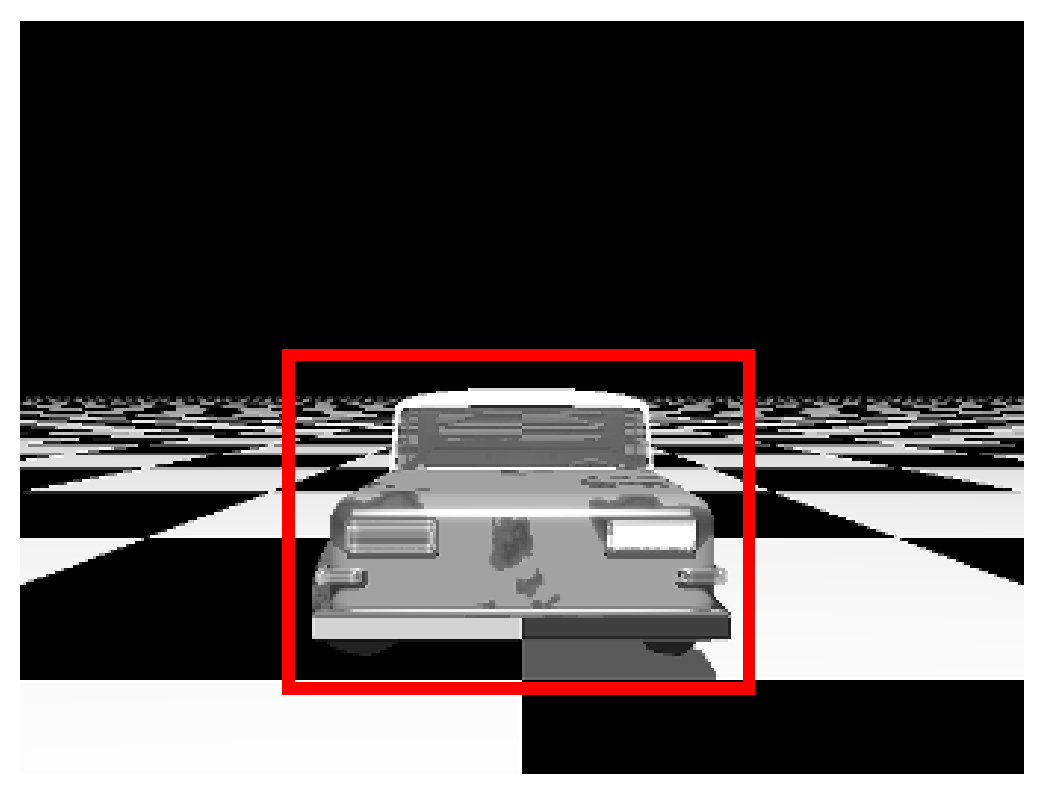
\includegraphics[width=.48\columnwidth]{images/figureb.eps}}
  \caption{The target in (a) is the initial position and its area is smaller than the target in (b), 
  which represents the final position. The factor is dividing both areas.}
  \label{fig:target}
\end{figure}

In Fig. \ref{fig:target}, we can observe an increase in ROI, and 
its influence to the departure factor is shown in Fig. \ref{fig:res_grapha_b}.

\begin{figure}[H]
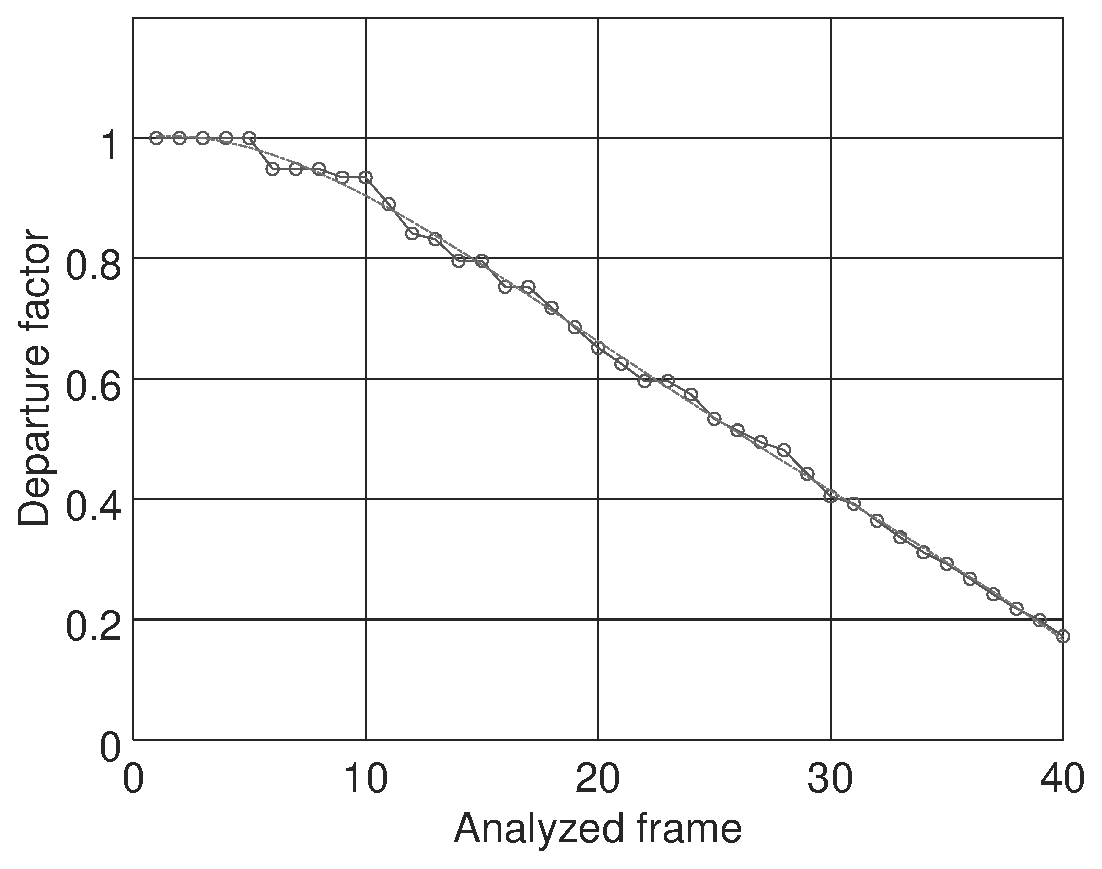
\includegraphics[width=\columnwidth]{images/grapha_b.eps}
\caption{Departure factor for each frame in the test 2.}
\label{fig:res_grapha_b}
\end{figure}

The Fig. \ref{fig:res_grapha_b} shows the departure factor in each frame
of test 2 (see the line with circles), additionally It is showed a polynomial
fitting of departure factor using a polynomial of order 4 (see the line with dots),
finally It is showed the real route of target normalized to $1.0$ for the maximum distance
(see the line with squares), as can be seen the target is approaching with a constant speed. 
If we interpret this value as the position in each sample time, 
then the departure factor describes the relative target position.
In the first image the analyzed target is at a distance $d_0$ 
and in the last image the target is at a distance of $17.18\%$ of $d_0$.
The departure distance decreases in discrete steps because the departure
factor is selected in discrete steps, if the target is
between two consecutive analysis layers (scales), the algorithm
approximates the target to the nearest layer.



The Table \ref{tab:tab1} represents the bank of images used for test 2, totally 40 images generated by POV-Ray.
The number of analyzed frames are in the first column of table, in the second column are the real distances 
between camera and target.
The percentage proportion of real distances are in third column. For example, 
the target in first frame is to $23.5$ meters from camera and it is considered the $100$\% of distance,
by other side, in the frame $40$ the target is to $4$ meters 
from camera and is $17,02$\% in relation of first frame. Next column, fourth column, 
we have the results of algorithm (departure factor), in the percentage form. 
%Note in first frame, target is $100$\% of distance and the last frame is at $17,18$\% of distance in relation of first frame.
Finally, the last column represents the error between percentage real distance and the departure factor. 
As can be seen, the error is diminishing when target is close (around 5 meters), it means that the algorithm has more precision 
when image of target is bigger because there are more information in ROI. It is a consequence of CCP, 
because in small ROI each pixel charge much information in comparative method. On other hand, if ROI is bigger,
the information is diluted around pixels; thus, the algorithm has more data to compare.
Another reason is that in the last frames $1$ pixel of target
represents a less distance in meters that $1$ pixel in the target of the first frames; consequently, the error 
of a quantity $x$ of pixels represents a less quantity of error meters in the analysis of last frames.

\begin{table}[H]
\setlength{\tabcolsep}{1 pt} 
\caption{Table of comparative results}
\begin{tabular}{lllll}
Frames & Real Dist. (m) & Real Dist. (\%) & Dep. factor (\%) & Relative error (\%)\\
1 & 23.5 & 100.0 & 100.0 & 0.0 \\
10 & 19.0 & 80.85 & 93.46 & 15.60 \\
20 & 14.0 & 59.57 & 65.16 & 9.37 \\
30 & 9.0 & 38.30 & 40.46 & 5.65 \\
40 & 4.0 & 17.02 & 17.18 & 0.93
\end{tabular}
\label{tab:tab1}
\end{table}

The Fig. \ref{fig:res_grapha_bv} shows the velocities of the data showed in the 
Fig. \ref{fig:res_grapha_b}  calculated to $d_0=1$ and $\Delta t=1$. 
Thus, it is showed the velocity of departure factor (see the line with circles), 
additionally It is showed the velocity of the polynomial
fitting of departure factor (see the line with dots) and
finally It is showed the velocity of the normalized real route
(see the line with squares), being it a constant.
The velocities were calculated using the discrete-time derivate.
The values of the velocities are negatives, which indicates that the
target is approaching towards the observer. As can be seen,
the velocity of the departure factor don't have a monotone behavior 
because that the curve of the departure factor has a many discrete changes; thus,
It is important to use the polynomial fitting curve
to calculate the velocity, because this curve represents
very close the behavior of the velocity of the normalized real route.

\begin{figure}[!hbt]
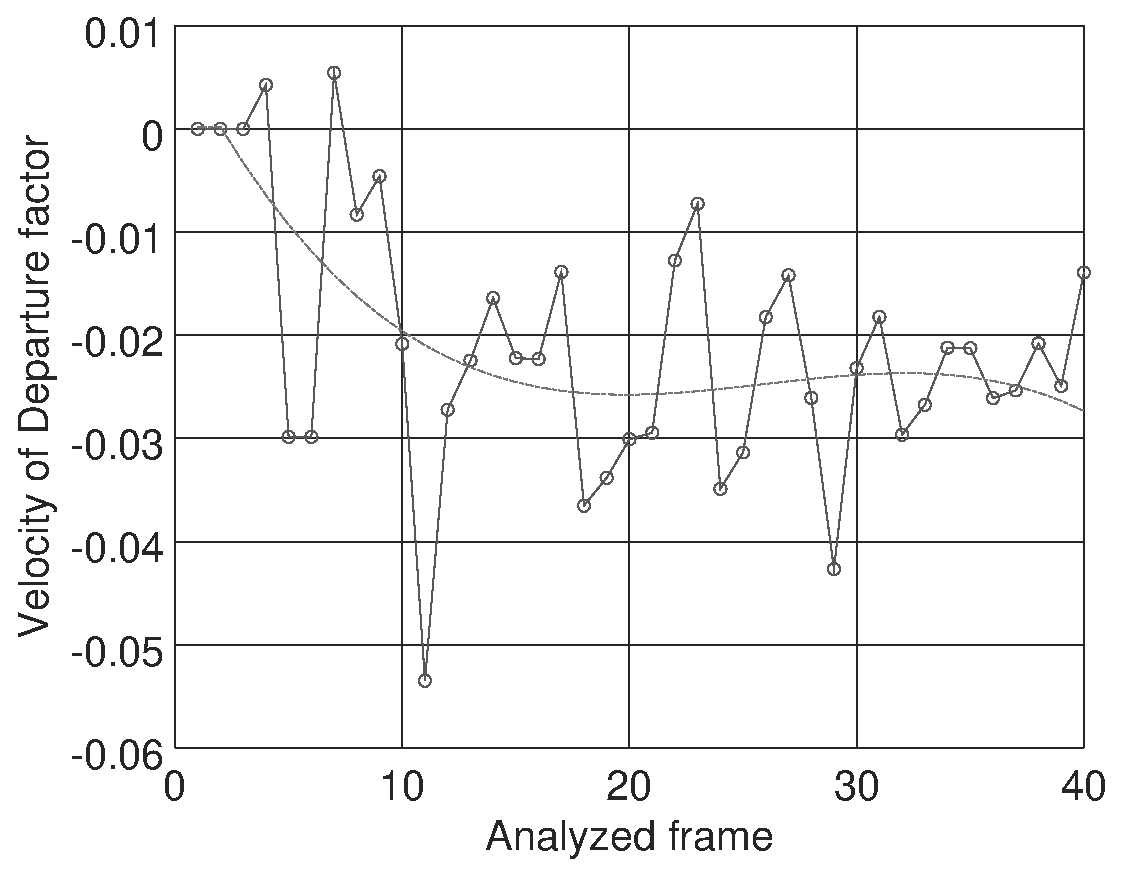
\includegraphics[width=\columnwidth]{images/graphvelocity.eps}
\caption{Velocity of departure factor for each frame in test 2.}
\label{fig:res_grapha_bv}
\end{figure}

\end{comment}


%%%%%%%%%%%%%%%%%%%%%%%%%%%%%%%%%%portugues%%%%%%%%%%%%%%%%%%%%%%%%%%%%%%%%%%%%%%%%%%%%%%%%
A funcionalidade do algoritmo para um caso em $3D$ é verificada no segundo teste;
nele, similar ao primeiro teste, o algoritmo compara um conjunto de imagens 
e calcula o fator de aproximação; porém, neste caso, o objeto de interesse tem um movimento
relativo em direção ao observador. A Figura \ref{fig:target} representa o 
rastreamento  do objeto de interesse em um fluxo de 40 imagens sequenciais. Os retângulos vermelhos
são as posições das regiões de análise inicial e final.

\begin{figure}[H]
\centering
  \subfloat[]{\label{fig:targeinit} 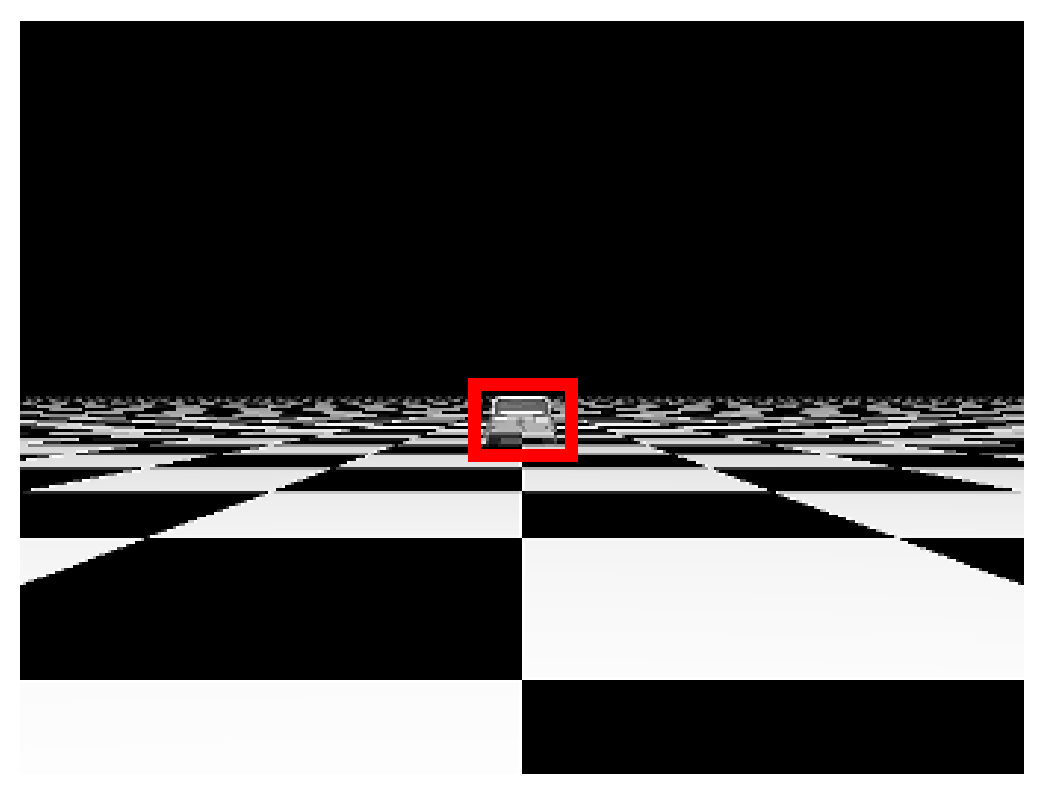
\includegraphics[width=.48\columnwidth]{images/figurea.eps}}
  \subfloat[]{\label{fig:targeend} 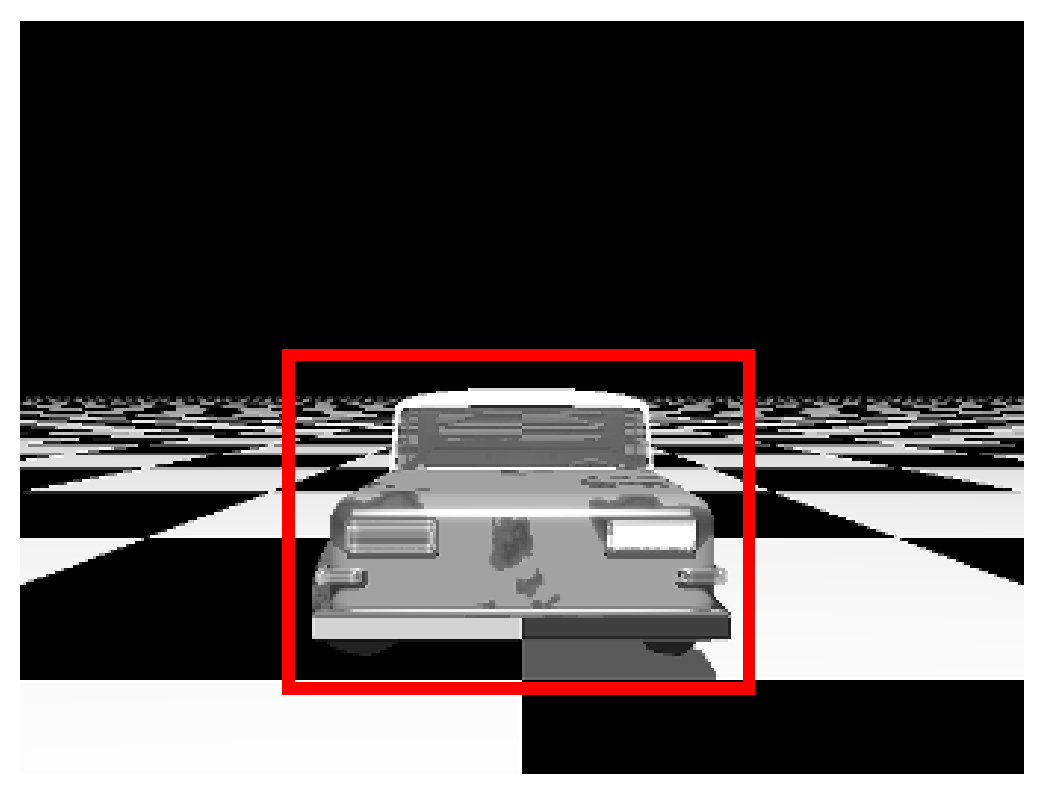
\includegraphics[width=.48\columnwidth]{images/figureb.eps}}
  \caption{O Objeto de interesse em (a) está na posição inicial com área menor que em (b), 
  a posição final.}
  \label{fig:target}
\end{figure}

Na Figura \ref{fig:target}, observa-se um crescimento na $ROI$ e, por
consequência, uma modificação do fator de aproximação $\beta$ relativo a $d_0$.
A Figura \ref{fig:res_grapha_b} apresenta o fator $\beta$ para cada uma das imagens 
do teste 2 (representado na linha com círculos).
Além disso, um ajuste polinomial deste fator a partir de um polinômio de ordem 4 é apresentado na linha pontilhada.
Finalmente, na linha com quadrados, é apresentada a distância normalizada entre o objeto de interesse e o observador,
de modo que a distância inicial $d_0=1.0$.
Como pode ser visto, o alvo está se aproximando com uma velocidade constante.
\begin{figure}[H]
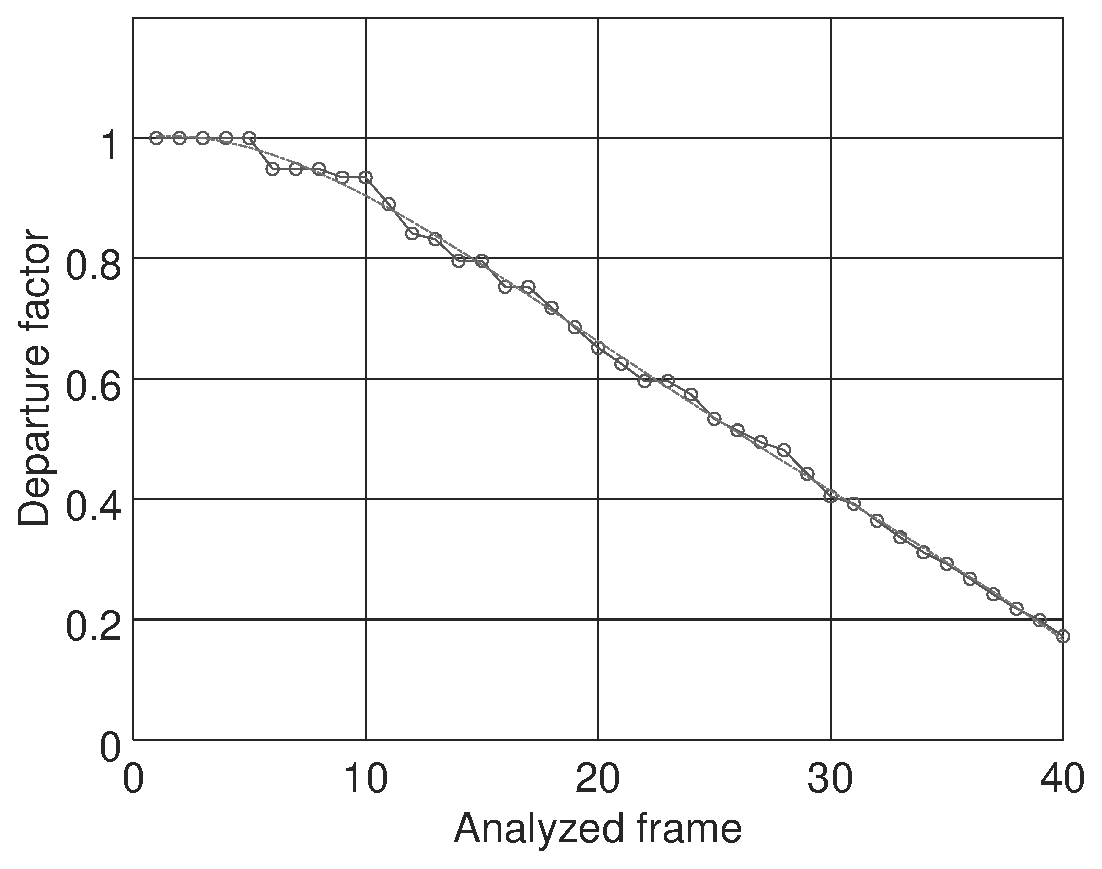
\includegraphics[width=\columnwidth]{images/grapha_b.eps}
\caption{O fator de aproximação $\beta$ relativo a $d_0$, para cada uma das imagens do teste 2.}
\label{fig:res_grapha_b}
\end{figure}


A tabela \ref{tab:tab1} descreve o resultado da análise do banco 
de imagens usado no teste 2, sendo um total de 40 imagens geradas
pelo programa de simulação POV-Ray.
\begin{table}[H]
\setlength{\tabcolsep}{1 pt} 
\caption{Tabela de resultados}
\begin{tabular}{l|l|l|l|l}
Imagem & Real Dist.(m) & Real Dist.(\%) & Fator de aprox.(\%) & Erro relativo(\%)\\ \hline  \hline
1 & 23.5 & 100.0 & 100.0 & 0.0 \\ \hline
10 & 19.0 & 80.85 & 93.46 & 15.60 \\ \hline
20 & 14.0 & 59.57 & 65.16 & 9.37 \\ \hline
30 & 9.0 & 38.30 & 40.46 & 5.65 \\ \hline
40 & 4.0 & 17.02 & 17.18 & 0.93 \\ \hline
\end{tabular}
\label{tab:tab1}
\end{table}
A primeira coluna representa o número da imagem analisada, e por uma questão de espaço, foram selecionados 
os resultados a cada 10 imagens; a segunda coluna contém a distância 
real em metros entre o objeto de interesse e o observador.
A porcentagem da distância real com $d_0$ está representada na terceira coluna. Por exemplo, o objeto na primeira imagem
está a $23.5$ metros da câmera, por outro lado, na imagem 40 o objeto está a
$4$ metros da câmera, apresentando uma distância de  $17,02$\% em relação a 
primeira imagem. Na quarta coluna estão os resultados do algoritmo (fator
de aproximação $\beta$ relativo a $d_0$) em porcentagem. Finalmente, a última coluna representa o erro 
entre a porcentagem da distância real e $\beta$.

Dado que é adotado um valor normalizado de $d_0=1,0$ como a posição do objeto de interesse na primeira 
imagem, então o fator de aproximação $\beta_i$ na imagem $I_i$ é 
numericamente igual a $d_i$, e descreve a posição relativa do objeto.
Assim, na primeira imagem o objeto analisado está a uma distância $d_0$
e na última imagem a uma distância $d_{40}=17.18\%d_0$.

É importante ressaltar que a aproximação do objeto à câmera é analisada de forma discreta, 
portanto, se o objeto
estiver entre duas camadas da análise, o algoritmo aproxima o resultado para
a camada mais próxima. Estas camadas são geradas pelo uso do fator $\alpha$
descrito no algoritmo \ref{alg:multires}. Outra consequência desta discretização
é a dificuldade de medir deslocamentos horizontais ou verticais, ou aumentos laterais da região de análise,
menores a $1$ pixel, de modo que quanto maior for a quantidade de pixels por
imagem analisada melhor será o desempenho do algoritmo para deslocamentos ou variações de área.

Um ponto a ser ressaltado é a diminuição do erro para distâncias próximas a 5 metros.  
Os resultados mostram que o algoritmo tem mais precisão conforme o objeto de interesse 
aumenta de área na imagem; pois este contém mais pixels (informação)
para os cálculos e, adicionalmente, cada pixel no objeto de interesse 
representa uma quantidade menor de metros na cena, de modo que
o erro em metros diminui.
Assim, no método de comparação ($CCP$), nota-se que quanto menor for a $ROI$ 
maior será o impacto do erro em cada pixel da imagem, 
e por consequência, menor precisão na descrição do objeto de interesse. 
Contudo, se o objeto de interesse cresce de tamanho na cena,
o método terá regiões de analise com mais informação (mais pixels), e menor porcentagem de metros do objeto por pixel,
o que leva a ter um erro em metros mais controlado, conforme pode se constatar nos testes realizados. 

A Figura \ref{fig:res_grapha_bv} apresenta a velocidade dos dados da 
Figura \ref{fig:res_grapha_b}, calculados para $d_0=1$ e $\Delta t=1$.
Assim, a velocidade do fator $\beta$ (linha com círculos) é ajustada por um polinômio
normalizado (linha pontilhada), segundo o percurso real do objeto (linha com quadrados).
A velocidade relativa do objeto foi calculada usando a derivada
discreta, sendo que os valores negativos indicam que o objeto está
em direção ao observador.

Para calcular a velocidade é necessário usar um ajuste polinomial devido 
as mudanças abruptas e erros causados pela discretização dos dados pelo fator $\beta$.
Assim, obtém-se uma descrição mais próxima da velocidade relativa do 
objeto de interesse.

\begin{figure}[H]
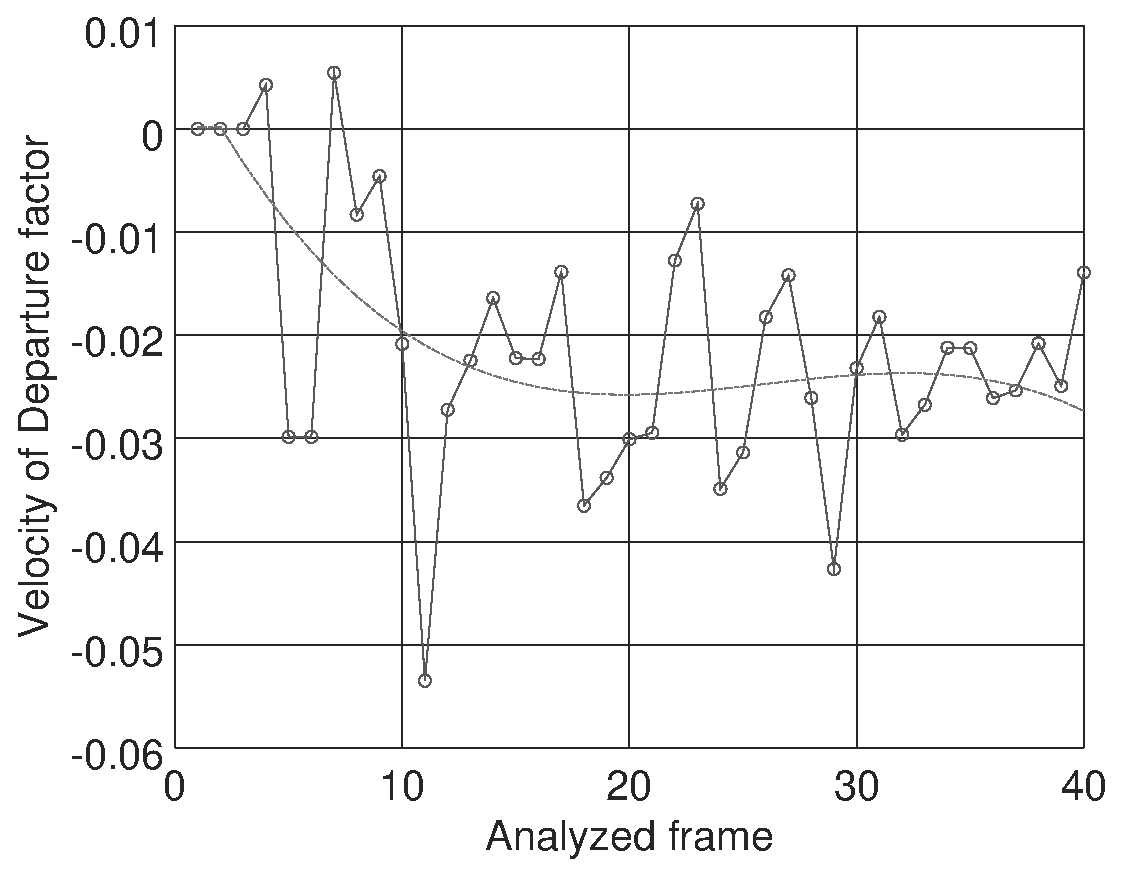
\includegraphics[width=\columnwidth]{images/graphvelocity.eps}
\caption{Velocidade das curvas normalizadas para cada um dos resultados obtidos no teste 2.}
\label{fig:res_grapha_bv}
\end{figure}
